\appendix

\section{Video Figure}

Please find a 2-minute overview of the functionality of our project here:\\ 
\href{https://www.youtube.com/watch?v=PPx2JuhQ9Us}{https://www.youtube.com/watch?v=PPx2JuhQ9Us}

\section{Individual Contributions}

\subsection{Rishav's Contributions}

\begin{figure}[htp]
    \centering
    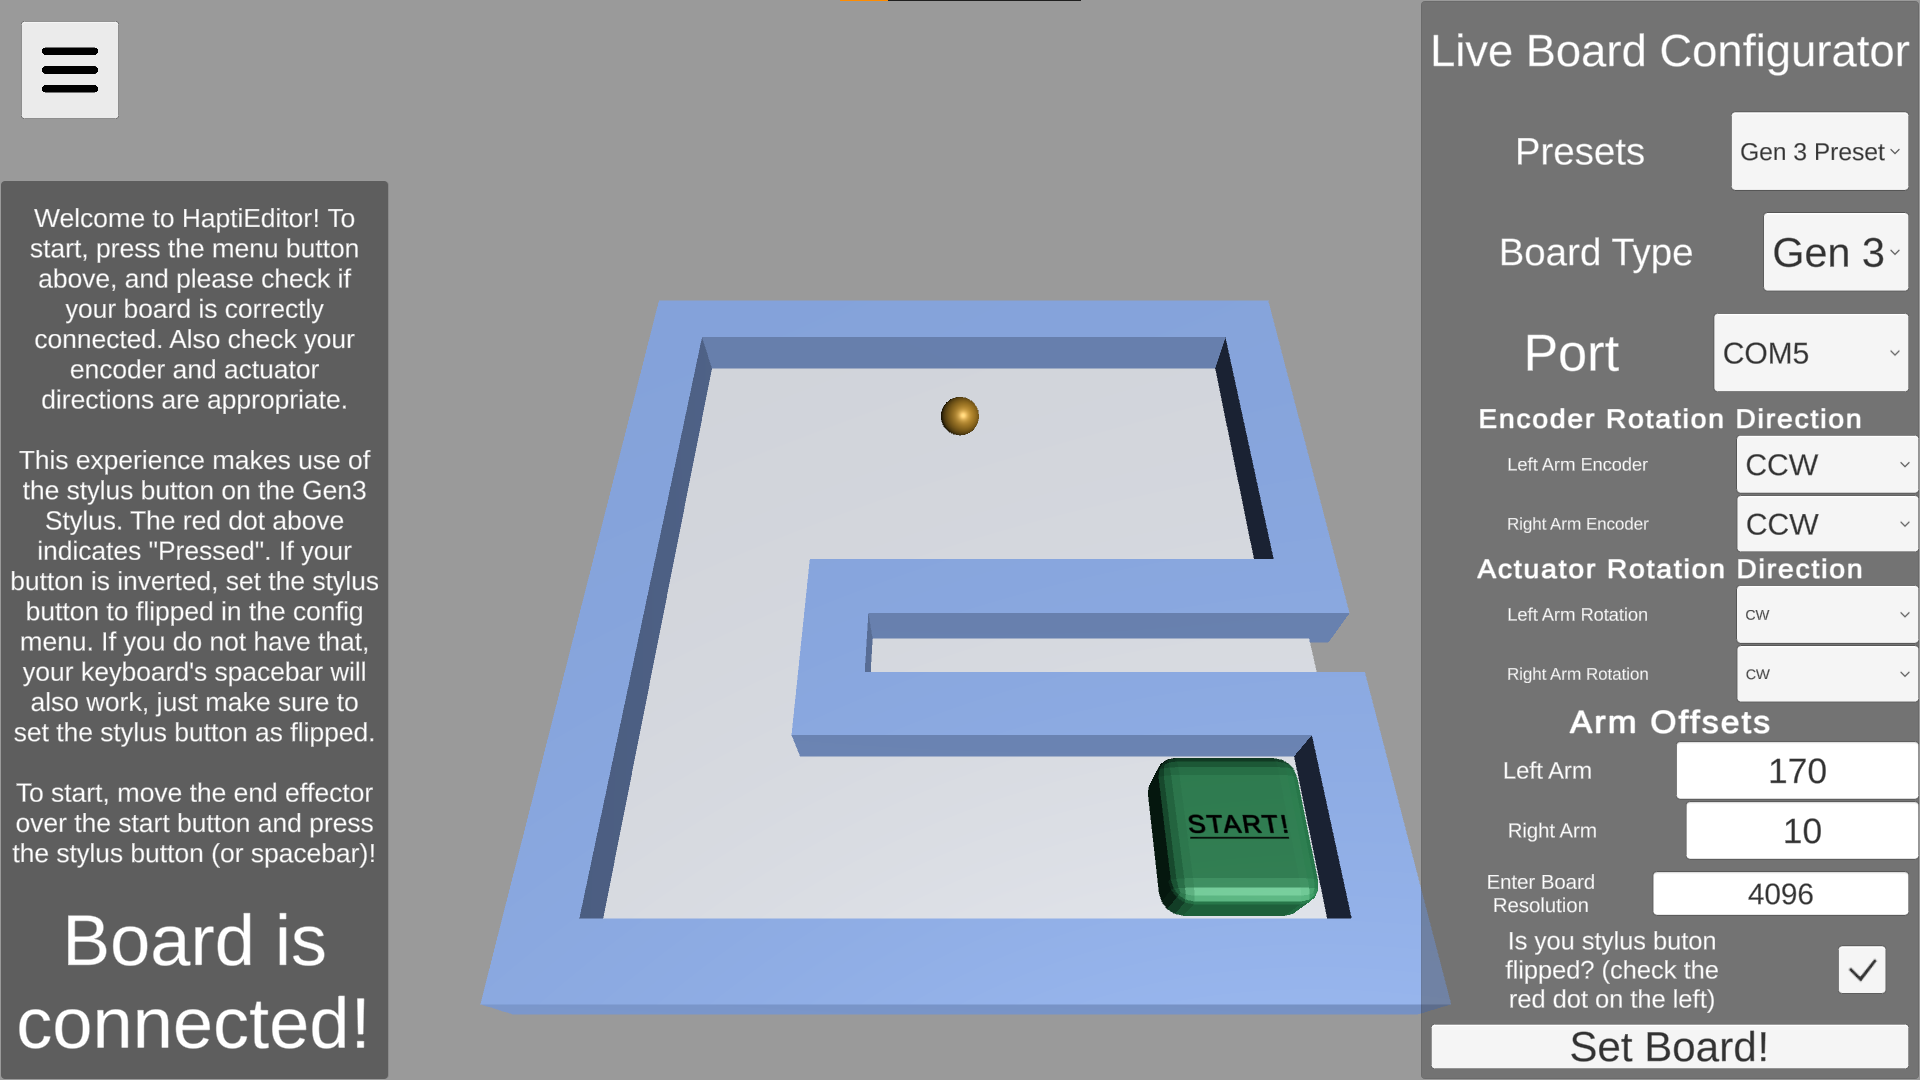
\includegraphics[width=14cm]{images/appendix-menu.png}
    \caption{HaptiEditor configuration menu}
    \Description{HaptiEditor configuration menu}
    \label{fig:menu}
\end{figure}

For the final iteration, we wanted to build an executable that anyone with a haply 2diy board can plug and play. Expecting everyone to install Unity would be quite an ask, so we needed to build a live board configurator.

The live board configurator would need to modify the following parameters:
\begin{itemize}
    \item Board Presets
    \item Gen2 or Gen3 (for arm distance offset)
    \item Encoder rotation direction
    \item Actuator rotation direction
    \item Arm offsets for base position
    \item Encoder resolution
    \item Flipped Stylus Button (Some Gen3 boards have flipped sensor data for the stylus port)
\end{itemize}

Actually passing the appropriate data and reloading the board was significantly more difficult. In a nutshell, I had to do the following:
\begin{itemize}
    \item Cancel the worker thread simulation task gracefully
    \item Flush all forces
    \item Delete the existing instance of the board (along with the encoder, actuator and sensor parameters)
    \item Create a new board instance with the new parameters
    \item Attempt a connection to the new specified port based on the user’s selection from current active ports
    \item Launch a new worker thread.
    \item Potentially connect to a Button Handler if the scene had one present.
\end{itemize}

This required a significant amount of refactoring of the core hAPI, but in the end I was successfully able to load and reload new user specified board configurations. The main chunk of this was happening in the \texttt{EndEffectorManager.cs} as follows:

\begin{minted}[style=friendly, linenos,fontsize=\footnotesize]{csharp}
public void ReloadBoard(DeviceConfig customConfig, string targetPort)
{
    // Destroying existing setup
    haplyBoard.DestroyBoard(); // added function to close port and destroy this board
    CancelSimulation();
    SetForces(0f, 0f);
    Destroy(pantograph.gameObject.GetComponent<Device>());
    // New Setup
    device = pantograph.gameObject.AddComponent<Device>();
    device.Init(); // re-establishes basic connections with pantograph and board
    LoadBoard(customConfig, targetPort);
    // Checking for button handler
    ButtonHandler buttonHandler = gameObject.GetComponent<ButtonHandler>();
    if (buttonHandler == null) return;
    buttonHandler.SetButtonState(customConfig.FlippedStylusButton);
}

private void LoadBoard(DeviceConfig customConfig = null, string targetPort = null)
{
    device.LoadConfig(customConfig);   // loads new config if custom config is not null
    haplyBoard.Initialize(targetPort); // attempts connection with new port
    device.DeviceSetParameters();
    // ...
    simulationLoopTask = new Task( SimulationLoop );
    simulationLoopTask.Start();
}
\end{minted}

After this, I decided to improve the visual experience of the project. Users will be expected to understand that they have to configure their board, and that their board might be set up different to our dev setups, so the menu scene should ideally be different from the actual terrain editing scene. Additionally, the stylus button (or space bar) is critical to the experience, so the users should be aware of how to do that as well.

To let the user learn this separately, I worked on a simple menu scene with a bit of flair, and added scene transitions. Users will now be expected to first configure their board, be able to move over a physical button in the world, and then click on the stylus button to enter the terrain painter tool.

I fished out a basic scene manager and transition handler from an older project, and after some tweaking, blender modelling and building an executable for Windows, I produced the menu scene in \autoref{fig:menu}.

\subsection{Sean's Contributions}

This iteration, I finalized work on the texture pipeline and integrated it with Pierre’s work from iteration 2 on texture and object painting on the terrain object. Pierre wrote some logic to get world position into a corresponding position on the surface of the terrain object, removing the need for our expensive physics ray-cast. The rest of the process involved the following changes:

\begin{itemize}
    \item Detecting which terrain texture was currently painted onto the surface of the terrain underneath the end effector. This required fetching the blend ratios of each material at the EE location and determining which was present:

          \begin{minted}[style=friendly, linenos,fontsize=\footnotesize]{csharp}
float[,,] swatch = terrain.terrainData.GetAlphamaps((int)pixelUV.x, (int)pixelUV.y, 1,1);
\end{minted}

    \item Once I have the ID of the texture to sample, we fetch color from its normal texture, giving us both a direction and intensity of force we immediately apply to our end effector. This greatly simplified the sampling code:

          \begin{minted}[style=friendly, linenos,fontsize=\footnotesize]{csharp}
Color normalPixel = prot.normalMap.GetPixel((int)normalUV.x, (int)normalUV.y);

forces.x += normalPixel.r - 0.5f
forces.y += normalPixel.g - 0.5f;

forces *= intensity;
previousPosition = eeTransform.position;
\end{minted}

    \item  I introduced a variable \texttt{swatchscale} to allow us to control the ratio of world movement relative to movement on the normal map, controlling the linear density of our texture. Normal sampling also greatly improved the accuracy of forces, as we’re no longer estimating heightmaps from surface color but now have geometry-accurate normal maps.
    \item  Selected texturally distinct normal maps for our materials for a clearer distinction between painted materials.
    \item  Added back space-bar support for painting, so a user has an alternative to the stylus button.
\end{itemize}

I then tuned the scaling code Rishav worked on in iteration 2 and added it to our scene. The following changed:

\begin{itemize}
    \item I added a scale factor for the movement range of the end effector, so it expanded as the scene zoomed out, covering the new area.
    \item I then tuned the ratios for movement range, end effector size and camera zooming so that they scaled in tandem.
    \item I changed the painter code so that the painted objects had their appropriate colliders, allowing the large end effector to skate over rocks as we’d intended it to, rather than getting stuck like before.
\end{itemize}

Lastly, I tuned the texture sampling code again so that it would play nice with the zooming feature we’d introduced. I chose a \texttt{swatchscale} such that at high zoom levels, individual surface features like pebbles were quite large and discernible, but with a wider camera, surface features became higher frequency noise and force feedback from geometry became the primary force on the end effector. Textures representations were different depending on the painted texture on the terrain and could be rendered in tandem with terrain objects placed during use. We learned that these pipelines could all coexist in a cohesive way and were pleased to see our parallel approach to developing them paid off.

Post iteration 3, I fixed some outstanding bugs, worked on my section of the report, and prepared the video figure.

\subsection{Pierre's Contributions}
As stated in our blog posts for iteration 2, the goal for the third was to merge every concepts and prototypes into one single, preferably enjoyable, experience. In this iteration we ended up working together way more and in closer collaboration by helping each others a lot more. This can be easily explained because we didn’t prototype on a different aspect of the experience and were actually making something unique together. This is why sometimes the lines of contributions of what I did and what a team member did will blur into what we did this feature together.

While we knew that we would merge all of our progress into the Terrain scene because the end goal is to use Unity’s Terrain game object has our editor, the \texttt{TerrainScript.cs} from iteration 2 wasn’t usable as is. Firstly, we need to fix the lack optimizations. Secondly, the user should have a way to change the brush type and their specifics without using Unity editor menus (it is necessary if the user interacts with our software through an executable instead of the Unity Project). Thirdly, Lastly, it is unlikely the code we used for texture sampling for haptic feedback would work on the Terrain game object, because it has the particularity to not have a \texttt{MeshRenderer} (a component that allows a game object to render a mesh). Finally, there needs to be a way paint using the stylus button instead of the mouse.

During this iteration Rishav did an amazing work at going over the code that has been made and telling us what should be avoided in the future. Following those practices we started a refactoring on \texttt{TerrainScript.cs}.  During this time, I found a way to optimize the management of the \texttt{TreeInstances} what were giving us issues during the second iteration, basically, deleted \texttt{TreeInstances} would never really be deleted but replaced with empty version of themselves.

This is problematic because with the core logic of the problem they would be given another collider the next time the software is running even though there is nothing to delete.

\begin{minted}[style=friendly, linenos,fontsize=\footnotesize]{csharp}
private void OnApplicationQuit()
{
    //test
    List<TreeInstance> trees = new List<TreeInstance>(terrain.terrainData.treeInstances);
    List<TreeInstance> trees_cleaned = new List<TreeInstance>();
    TreeInstance empty_tree = new TreeInstance();
    for (int i = 0; i < trees.Count; i++)
    {
        if (!trees[i].Equals(empty_tree))
            trees_cleaned.Add(trees[i]);
    }
    terrain.terrainData.SetTreeInstances(trees_cleaned.ToArray(), true);
}
\end{minted}

Using this code when the application is closed we remove all of the \texttt{TreeInstances} that we could consider empty. The way it works is by going through all the objects in the Terrain \texttt{TreeInstances}  and comparing it with an empty object. If they are different we add them to the new list that will contain all the non-empty \texttt{TreeInstance}.

Then using the \texttt{ObjectPlacer.cs} as a reference I created two co-routines one for painting object on the terrain and the other for painting texture. We implemented an enumerator containing all the brushes types (i.e. Texture, Object and Object Eraser) and depending on this brush type one of the co-routine or the object deletion will be enabled.

From then on Rishav worked with me on a basic UI so we can change the brush types and which texture/object is being painted.

\subsection{Previous Iterations}
